\documentclass{beamer}
\mode<presentation>
\usepackage{amsmath,amssymb,mathtools}
\usepackage{textcomp}
\usepackage{gensymb}
\usepackage{adjustbox}
\usepackage{subcaption}
\usepackage{enumitem}
\usepackage{multicol}
\usepackage{listings}
\usepackage{url}
\usepackage{graphicx} % <-- needed for images
\def\UrlBreaks{\do\/\do-}

\usetheme{Boadilla}
\usecolortheme{lily}
\setbeamertemplate{footline}{
  \leavevmode%
  \hbox{%
  \begin{beamercolorbox}[wd=\paperwidth,ht=2ex,dp=1ex,right]{author in head/foot}%
    \insertframenumber{} / \inserttotalframenumber\hspace*{2ex}
  \end{beamercolorbox}}%
  \vskip0pt%
}
\setbeamertemplate{navigation symbols}{}

\lstset{
  frame=single,
  breaklines=true,
  columns=fullflexible,
  basicstyle=\ttfamily\tiny   % tiny font so code fits
}

\numberwithin{equation}{section}

% ---- your macros ----
\providecommand{\nCr}[2]{\,^{#1}C_{#2}}
\providecommand{\nPr}[2]{\,^{#1}P_{#2}}
\providecommand{\mbf}{\mathbf}
\providecommand{\pr}[1]{\ensuremath{\Pr\left(#1\right)}}
\providecommand{\qfunc}[1]{\ensuremath{Q\left(#1\right)}}
\providecommand{\sbrak}[1]{\ensuremath{{}\left[#1\right]}}
\providecommand{\lsbrak}[1]{\ensuremath{{}\left[#1\right.}}
\providecommand{\rsbrak}[1]{\ensuremath{\left.#1\right]}}
\providecommand{\brak}[1]{\ensuremath{\left(#1\right)}}
\providecommand{\lbrak}[1]{\ensuremath{\left(#1\right.}}
\providecommand{\rbrak}[1]{\ensuremath{\left.#1\right)}}
\providecommand{\cbrak}[1]{\ensuremath{\left\{#1\right\}}}
\providecommand{\lcbrak}[1]{\ensuremath{\left\{#1\right.}}
\providecommand{\rcbrak}[1]{\ensuremath{\left.#1\right\}}}
\theoremstyle{remark}
\newtheorem{rem}{Remark}
\newcommand{\sgn}{\mathop{\mathrm{sgn}}}
\providecommand{\abs}[1]{\left\vert#1\right\vert}
\providecommand{\res}[1]{\Res\displaylimits_{#1}}
\providecommand{\norm}[1]{\lVert#1\rVert}
\providecommand{\mtx}[1]{\mathbf{#1}}
\providecommand{\mean}[1]{E\left[ #1 \right]}
\providecommand{\fourier}{\overset{\mathcal{F}}{ \rightleftharpoons}}
\providecommand{\system}{\overset{\mathcal{H}}{ \longleftrightarrow}}
\providecommand{\dec}[2]{\ensuremath{\overset{#1}{\underset{#2}{\gtrless}}}}
\newcommand{\myvec}[1]{\ensuremath{\begin{pmatrix}#1\end{pmatrix}}}
\let\vec\mathbf

\title{MatGeo Presentation - Problem 3.2.5}
\author{EE25BTECH11064 - Yojit Manral}
\date{}

\begin{document}

\frame{\titlepage}
\begin{frame}{Question}
Draw a triangle ABC in which BC = 6 cm, CA = 5 cm and AB = 4 cm.\\
\end{frame}

\begin{frame}{Solution}
$\rightarrow$ Let
\begin{align}
    a = \norm{\vec{C} - \vec{B}} = 6 cm \\
    b = \norm{\vec{A} - \vec{C}} = 5 cm \\
    c = \norm{\vec{B} - \vec{A}} = 4 cm
\end{align}
$\rightarrow$ By using cosine law in $\triangle$ABC, we get
\begin{align}
    &\cos{B} = \frac{a^{2} + c^{2} - b^{2}}{2ac} \\
    \implies &\cos{B} = \frac{6^2 + 4^2 - 5^2}{2 \times 6 \times 4} \\
    \implies &\cos{B} = \frac{9}{16} \\
    \implies &\angle{B} = \cos^{-1}{\brak{\frac{9}{16}}} \approx 55 \degree
\end{align}
\end{frame}

\begin{frame}{Solution}
$\rightarrow$ The coordinates of $\triangle$ABC can then be expressed as
\begin{align}
    \vec{A} = c \myvec{\cos{B}\\\sin{B}} &&
    \vec{B} = \myvec{0\\0} &&
    \vec{C} = \myvec{0\\6} \notag
\end{align}

\begin{figure}[h!]
   \centering
   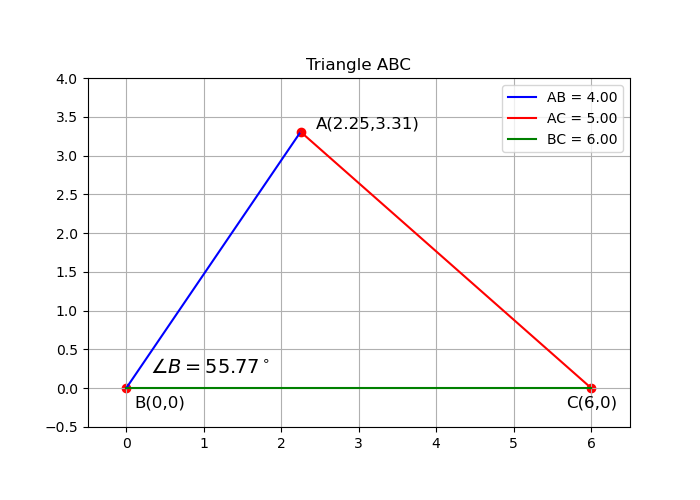
\includegraphics[width=0.6\linewidth]{figs/01.png}
   \caption{Plot of $\triangle$ABC}
   \label{Plot_1}
\end{figure}
\end{frame}
 % --------- CODE APPENDIX ---------
\section*{Appendix: Code}

% C program
\begin{frame}[fragile]{File: points.c}
\begin{lstlisting}[language=C]
#include <stdio.h>

int main() {
  FILE *fp;

  // -------------------
  // Question 3.2.5
  // -------------------


  fp = fopen("points.dat", "w");
  fprintf(fp, "%d,%d,%d\n", 2.25, 3.31, 0);  // A
  fprintf(fp, "%d,%d,%d\n", 0, 0, 0);   // B
  fprintf(fp, "%d,%d,%d\n", 6, 0, 0); // C
  fclose(fp);
  return 0;
}
\end{lstlisting}
\end{frame}

% Python calling C
\begin{frame}[fragile]{File: call\_c.py}
\begin{lstlisting}[language=Python]
import subprocess

# Compile the C program
subprocess.run(["gcc", "points.c", "-o", "points"])

# Run the compiled C program
result = subprocess.run(["./points"], capture_output=True, text=True)

# Print the output from the C program
print(result.stdout)
\end{lstlisting}
\end{frame}

% Python plotting
\begin{frame}[fragile]{File: plot.py}
\begin{lstlisting}[language=Python]
import matplotlib.pyplot as plt
import numpy as np

# Given coordinates
B = np.array([0, 0])
C = np.array([6, 0])
A_x = 4 * np.cos(np.deg2rad(55.77))  # A_x = 4 * cos(55.77 degrees)
A_y = 4 * np.sin(np.deg2rad(55.77))  # A_y = 4 * sin(55.77 degrees)
A = np.array([A_x, A_y])

# Calculate side lengths
AB = np.linalg.norm(A - B)
BC = np.linalg.norm(C - B)
AC = np.linalg.norm(A - C)

# Calculate angle B using the law of cosines
cos_angle_B = (AB**2 + BC**2 - AC**2) / (2 * AB * BC)
angle_B_rad = np.arccos(cos_angle_B)  # In radians
angle_B_deg = np.rad2deg(angle_B_rad)  # Convert to degrees

# Create the plot
plt.figure(figsize=(7, 5))

# Plot the triangle
plt.plot([B[0], A[0]], [B[1], A[1]], 'b-', label=f'AB = {AB:.2f}')
plt.plot([A[0], C[0]], [A[1], C[1]], 'r-', label=f'AC = {AC:.2f}')
plt.plot([C[0], B[0]], [C[1], B[1]], 'g-', label=f'BC = {BC:.2f}')
\end{lstlisting}
\end{frame}

% Python plotting
\begin{frame}[fragile]{File: plot.py}
\begin{lstlisting}[language=Python]
# Mark the vertices
plt.scatter([B[0], A[0], C[0]], [B[1], A[1], C[1]], color='red')
plt.text(B[0]+0.1, B[1]-0.1, 'B(0,0)', fontsize=12, ha='left', va = 'top')
plt.text(A[0]+0.2, A[1], f'A({A_x:.2f},{A_y:.2f})', fontsize=12, ha='left', va = 'bottom')
plt.text(C[0], C[1]-0.1, 'C(6,0)', fontsize=12, ha='center', va='top')

# Label the angle at B and its value
plt.text(B[0] + 0.3, B[1] + 0.2, r'$\angle B = {:.2f}^\circ$'.format(angle_B_deg), fontsize=14, ha='left')

# Set plot properties
plt.gca().set_aspect('equal', adjustable='box')
plt.xlim(-0.5, 6.5)
plt.ylim(-0.5, 4)

# Title and grid
plt.title('Triangle ABC')
plt.grid(True)

# Show the plot
plt.legend()
plt.show()

\end{lstlisting}
\end{frame}

\end{document}
